\documentclass[12pt]{article}

\usepackage{fullpage}
\usepackage{multicol,multirow}
\usepackage{tabularx}
\usepackage{ulem}
\usepackage[utf8]{inputenc}
\usepackage[russian]{babel}
\usepackage{graphicx}
\DeclareGraphicsExtensions{.png}

\renewcommand{\labelenumii}{\arabic{enumi}.\arabic{enumii}.}


\begin{document}

\section*{Лабораторная работа №\,2 по курсу криптографии}

Выполнила студентка группы М8О-307Б \textit{Довженко Анастасия}.

\subsection*{Условие}

\begin{enumerate} 
\item Сгенерировать OpenPGP-ключ и самоподписанный сертификат (например, с помощью дополнения Enigmail к почтовому клиенту thunderbird).
\item Установить связь с преподавателем и с хотя бы с одним одногруппником, используя созданный ключ, следующими действиями:
\begin{enumerate} 
\item Прислать от своего имени по электронной почте сообщение, во вложении которого поместить свой открытый ключ.
\item Дождаться письма, в котором отправитель вам пришлёт свой сертификат открытого ключа.
\item Выслать сообщение, зашифрованное на ключе отправителя.
\item Расшифровать письмо своим закрытым ключом.
\item Убедиться, что ключу абонента можно доверять путём сравнения отпечатка ключа или ключа целиком, по доверенным каналам связи.
\end{enumerate} 
\item Собрать подписи под своим ключом.
\begin{enumerate}
\item Подписать сертификат открытого ключа одногруппника и преподавателя своим ключом.
\item Выслать почтой сертификат полученный в п.3.1 его владельцу.
\item Собрать 10 подписей одногруппников под своим сертификатом.
\item Прислать преподавателю (желательно почтой) свой сертификат, с 10-ю или более подписями одногруппников.
\end{enumerate}
\end{enumerate}


\subsection*{Метод решения}
Файлы:\\
my\_key.asc -- мой ключ.\\
signed\_key.asc -- подписанный ключ преподавателя.\\
\newpage

Я сгенерировала ключ:\\
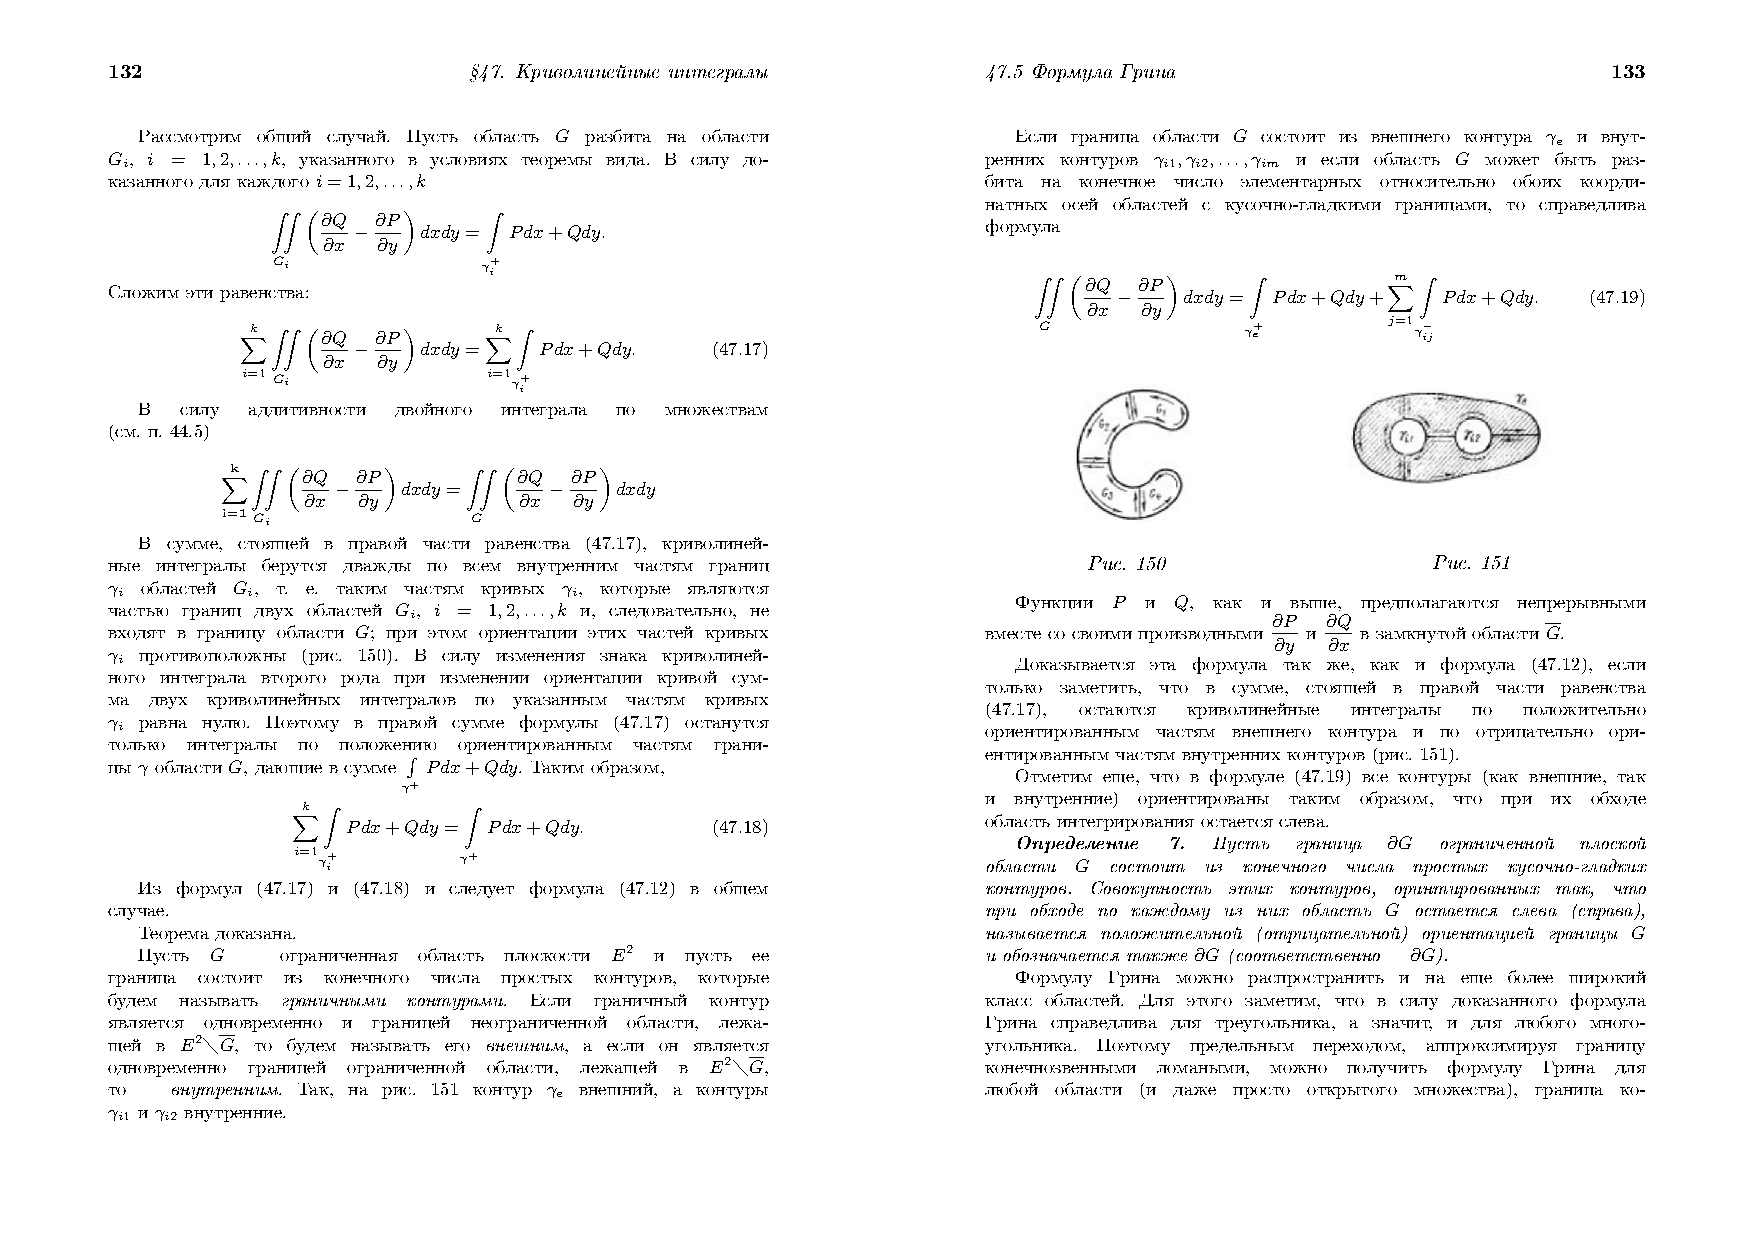
\includegraphics[width=\linewidth]{1.png}\\

Прислала свой открытый ключ одногруппнице:\\
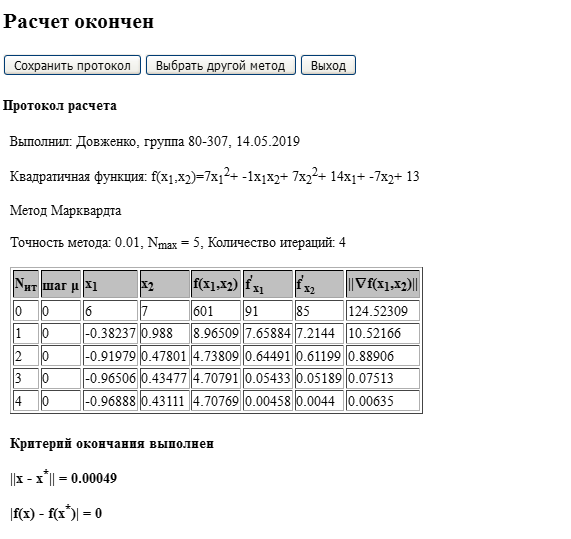
\includegraphics[width=\linewidth]{5.png}\\

Дождалась письма, в котором одногруппница прислала мне свой сертификат:\\
\includegraphics[width=\linewidth]{7.png}\\

Выслала сообщение, зашифрованное на ключе отправителя:\\
\includegraphics[width=\linewidth]{8.png}\\
\newpage

Расшифровала полученное письмо своим закрытым ключом:\\
\includegraphics[width=\linewidth]{9.png}\\

Дальше я сравнила ключ в письме и ключ в менеджере ключей и нашла соответствие:\\
\includegraphics[width=\linewidth]{10.png}\\
\includegraphics[width=\linewidth]{11.png}\\

Также я отправила свой открытый ключ и зашифрованное сообщение преподавателю:\\
\includegraphics[width=\linewidth]{12.png}\\
\includegraphics[width=\linewidth]{13.png}\\
\newpage

В конце я собрала 11 подписей однокурсников под своим сертификатом:\\
\includegraphics[width=\linewidth]{15.png}\\

\subsection*{Выводы}
Я научилась пользоваться шифрованием и подписью на примере pgp и почты. Основные сложности при выполнении работы были связаны с организационной частью: поначалу мало кто из моих однокурсников хотел участвовать в key signing party. Путем недолгих переговоров мне все-таки удалось убедить 11 человек подписать мой сертификат. В остальном это были монотонные шаблонные действия по пересылке сообщений.\\

Вообще механизм работы pgp показался мне интересным. Под капотом много классных алгоритмов шифрования, сжатия, хеширования. Наверно, интересно было бы написать прототип такой системы.

\end{document}
